 \documentclass[11pt,a4paper]{article}
\usepackage[utf8]{inputenc}
\usepackage[finnish]{babel}
\usepackage[T1]{fontenc}
\usepackage{amsmath}
\usepackage{amsfonts}
\usepackage{amssymb}
\usepackage{amsthm}
\usepackage{url}
\pagestyle{plain}
\usepackage{graphicx}
\title{Kolmen aineen analyysi}
\author{Delun Li\\014631300\\Orgaanisen kemian työt 1\\Työ 5}
\date{25.10.2018}

\begin{document}

\maketitle

\pagebreak


\section{Johdanto}

Tässä työssä annettiin liuos, jossa oli kolme eri orgaanista yhdistettä, tunnistettavaksi ja eristettäväksi.  Yhdisteet puhdistettiin tislaamalla tai uudelleenkiteyttämällä. Uuttamalla liuos ensiksi NaHCO$_3$:lla saadaan karboksyylihappo yhdisteet eristettyä liuoksesta vesikerrokseen suoloina ja sitten NaOH:lla saadaan fenolit ja HCl:lla amiinit eristettyä. Kaikkien kolmen uuttojen jälkeen uutetaan vesikerros eetterillä (30 ml), jotta voidaan varmistaa vesiliuoksen komponentin täydellisen erottumisen. Takaisinuutetut eetterit yhdistetään alkuperäiseen eetteriliuokseen.

\section{Esitestit}

Liuoksesta ajettiin IR-spektri ja tehtiin muutama osoitusreaktio ennen eristämistä. Happojen osoitukseksi käytettiin NaHCO$_3$:a, amiineja CuSO$_4$:a ja fenolia FeCl$_3$:a. Posittivsessa tilanteessa karboksyylihappotestissä liuos kuplii, amiinitestissä liuos muuttuu siniseksi tai vihreäksi tai muodostuu sakkaa ja fenolitestissä Fe$^{3+}$-ioni aiheuttaa värinmuutosta. Kaikista kokeista tuli negatiivinen tulos. 


\section{Työn suoritus}

Esitestien jälkeen liuostata uutettiin dietyylieetteriin (50 ml) ja sen jälkeen 2M NaHCO$_3$:lla (3x50 ml). Eetterifaasi uutettiin 2M NaOH:lla (2x50 ml) ja sitten 4M HCl:lla (3x40 ml). Talteen otettiin NaHCO$_3$:n (\textbf{1}), NaOH:n (\textbf{2}) ja HCl:n (\textbf{3}) vesiliuokset ja niiden uuttojen jälkeen jäänyt eetteriliuos (\textbf{4}).

Edellisten osoitusreaktioiden perusteella liuoksessa ei ole happoja, amiineja ja fenoleita, jolloin aloitettiin neutraali aineiden eristämistä liuoksesta \textbf{4}. Eetteriliuos kuivattiin MgSO$_4$:lla, jonka jälkeen tislattiin dietyylieetteri pois (kiehumispiste k.p $\approx$ 35$^\circ$C)$^1$. Seuraavaksi tislautui \textbf{neste 2} (k.p $\approx$ 75$^\circ$C) ja viimeisenä tislautui \textbf{neste 1} (k.p $\approx$ 152$^\circ$C). Tisleistä ajettiin IR- ja $^1$H-NMR-spektrit ja mitattiin taitekertoimet (\textbf{neste 2}$=$1.5154, \textbf{neste 1}$=$1,3905).

Tähän menneessä eristettiin mahdollisesti kahta eri neutraali ainetta, jolloin jäljelle jäi yksi tuntematon aine. Tehtiin liuokset \textbf{1} ja \textbf{2} happamiksi väkevällä HCl:lla ja liuos \textbf{3} emäksiseksi 40$\%$ NaOH:lla. Ainoastaan liuoksesta \textbf{2} näkyi visuaalista muutosta eli liuoksessa \textbf{2} oli mahdollisesti fenolia. Liuokseen \textbf{2} muodostui beigen väristä vaahota muistuttavaa sakkaa. Tällöin lähdettiin tutkimaan liuosta \textbf{2}.

Liuoksessa \textbf{2} oleva sakkaa, \textbf{kiinteä aine}, imusuodatettiin ja uudelleenkiteytettiin kiehuvasta vedestä. Kiinetästä fenolista ajettiin IR- ja $^1$H-NMR-spektrit ja mitattiin sulamispiste (120,6$^\circ$C). Eli siis tässä vaiheessa eristettiin mahdollisesti neutraali yhdisteet \textbf{neste 1} ja \textbf{neste 2} ja fenoli \textbf{kiinteä aine}. 

\section{Tuntemattomien aineiden analysointi}


\subsection{Neste 2}

Tutkimalla liitettä \textbf{IR-spektri: Etyyliasetaatti}, joka kuvaa \textbf{neste 2} IR-spektriä, huomataan spektrin olevan melko yksinkertainen. Spektrissä näkyy ensiksi kolme vahvaa piikkiä väliltä 1000-1750 cm$^{-1}$. 1730 cm$^{-1}$ tienoilla kuvaa mahdollisen karbonyyliryhmän C$=$O venytysvärähtelyä. Kuitenkin \textbf{neste 2} ei voi olla aldehydi, sillä 2720-2820 cm$^{-1}$:ssa ei löydy selvää kaksi piikkiä, jotka esittävät aldehydiryhmän C-H värähtelyä. Toisaalta välillä 1050-1250 cm$^{-1}$ olevat kaksi piikkiä kuvaavat mahdollisesti esterin C-O venytysvärähtelyä, jolloin \textbf{neste 2} ei todennäköisesti ole ketoni. Eli siis aaltoluvulla 1735 kuvaa mahdollisen esteriryhmän C$=$O venytysvärähtelyä. Tällöin voidaan sanoa yhdisteen sisältävän ainakin esteriryhmä. Absorbointeja ei löydy yli 3000 cm$^{-1}$:ssä keskivahvoja eikä 650-900 cm$^{-1}$:ssä vahvoja piikkejä, jotka kuvaisivat aromaattisen renkaan aiheuttamaa värähtelyä. 2850-2960 aaltoluvun välillä oleva absorbointi kuvaa mahdollisesti yhdisteen sp$^3$ sidoksia. $^{2}$ 

Liitteessä \textbf{$^1$H-NMR: Etyyliasetaatti}:ssa on \textbf{neste 2}:n $^1$-H-NMR-spektri. Spektristä nähdään selkeästi 3,30-3,90 ppm:ssä quartetti, 1,5 ppm:ssä singletti ja 0,5-0,9 ppm:ssä tripletti. Spektriä on tulkittu tarkemmin liitteesä \textbf{$^1$-H-NMR tulkinta: Etyyliasetaatti}. $^2$

IR- ja $^1$-H-NMR-spekrien lisäksi \textbf{neste 2} kiehumispiste (75$^\circ$C) ja taitekerroin (1,3738) ovat hyvin lähellä etyyliasetaatin kirjallisuuskiehumispistettä (77$^\circ$C) ja -taitekerrointa (1,3723).  $^{3,4}$ Voidaan sanoa \textbf{neste 2} olevan etyyliasetaatti. Varmistakseen verrattiin saatua IR- ja $^1$H-NMR-spektrejä kirjallisuuden$^{3,5}$. Spektrit näyttävät lähes identtisiltä. 

\subsection{Neste 1}

\textbf{Neste 1} IR-spektriä on kuvattu liitteessä \textbf{IR-spektri: Anisoli}. Spektrissä löytyy aromaattisen renkaan aiheuttamaa värähtelyä. 3030 cm$^{-1}$ ja 1660-2000 cm$^{-1}$ kuvavat aromaattista rengasta, 1450-1500 cm$^{-1}$ kuvaa renkaan C$=$C venytysvärähtelyä ja 730-770 cm$^{-1}$ ja 690-710 cm$^{-1}$ kuvaa renkaassa olevien viisi vierekkäisten vetyjen olemassaolosta. Aaltoluvun 1250 tienoilla esittää C-O värähtelyä. Verrattuna \textbf{neste 1} eli etyyliasetaatin IR-spektriä, huomataan \textbf{neste 2} spektrissä ei löydy C$=$O venytysvärähtelyä 1700 cm$^{-1}$ tienoilla. Tästä voidaan päätellä kyseinen C-O värähtely kuvaa eetteriryhmän kiinnittymistä aromaattiseen renkaaseen absorptio signaalia.  2850-2950 cm$^{-1}$:ssä esiintyvät absorptiot kuvaavat sp$^3$ sidosten värähtelyjä. $^2$

Toisaalta, kun analysoidaan liitettä \textbf{$^1$H-NMR: Anisoli}, joka kuvaa \textbf{neste 2} $^1$H-NMR-spektriä, huomataan vetysiirtymien sijoittuvan pitkälti 6,5-7,7 ppm:ssä ja 3,70 ppm:ssä. 7,0$\pm$0.5 ppm:ssä esiintyvät vetysiirtymät kuvaavat hyvin mahdollisesti aromaattisen renkaaseen kiinnittyneet vetyt ja 3,7 ppm:ssä oleva singletti kuvaa eristynyttä alkyyliä. Spektriä on analysoitu tarkemmin liitteessä \textbf{$^1$H-NMR tulkinta: Anisoli}.$^2$

\textbf{Neste 1} kiehumispisteeksi saatiin siis 152$^\circ$C ja taitekertoimeksi (1,5164). Nämä arvot ovat hyvin lähellä anisolin kirjallisuusarvoja$^{3,7}$ (k.p$=$155$^\circ$C, taitekerroin $=$1,51791). \textbf{Neste 2}:n spektreistä, kiehumispisteestä ja taitekertoimesta voidaan päätellä, että yhdiste on anisoli. Spektrejä verrattiin myös kirjallisuuden spektreihin$^{3,6}$ ja osoittautuivat näyttävän identtiseltä. 


\subsection{Kiinteä aine}

 Fenoliyhdisteen IR-spektrissä (liite: \textbf{IR: 2-naftoli)} huomataan fenolin -OH ryhmän aiheuttamaa venytystä 3000-3500 cm$^{-1}$ ja bentseeni renkaan aiheuttamaa venytystä aaltoluvuilla 3030, 1400-1600, 860-900, 800-860 ja 735-770. 860-900 cm$^{-1}$ kuvaa eristynyeen vedyn kiinittymistä renkaaseen, 800-860 kahden vierekkäisten vetyjen olemassaoloa ja 735-770 neljä vierekkäisten vetyjen olemassaolosta. 1400-1600 kuvaa renkaan sp$^2$ sidoksia. Näiden avulla voidaan päätellä, että yhdisteessä on mahdollisesti enemmän kuin yksi bentseeni rengas. $^2$

$^1$H-NMR spektrissä nähdään vetysiirtymiä 6,9-8,0 ppm:n kohdalla, jotka kuvaavat aromaattiseen renkaaseen kiinnittyneet vedyt, ja 5,0 ppm:n kohdalla -OH ryhmän vetysiirtymää. Spektrissä oleva siirtymä 1,55 ppm:n kohdalla on mahdollisesti käytetyn liuottimen, deuterokloroformin, aiheuttama kosteus, jolloin siirtymää ei oteta huomioon analysoinnissa.Liiteessä \textbf{$^1$H-NMR tulkinta: Anisoli} on analysoitu spektriä tarkemmin. $^2$

Mitattu sulamispiste (120,6$^\circ$C) on hyvin lähellä 2-naftolin kirjallisuusarvoa$^3$ (122$^\circ$C). Tämän lisäksi saadut spektrit ovat lähes identtisiä kirjallisuus-spektrien kanssa.$^{3,8,9}$

\section{Johtopäätökset}


Analysointien perusteella alkuperäisessä liuoksessa löytyy kiinteätä 2-naftolia ja nestemäistä etyyliasetaattia ja anisolia. Alla on esitetty kukin yhdisteen rakennemuoto. 

\vspace{0.3cm}

\hspace{-0.5cm}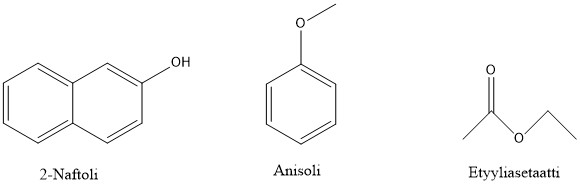
\includegraphics[width=12.5cm]{analyysi.jpg}

\vspace{0.3cm}

Aineiden eristys sujui melko ongelmitta. Ainoana haasteena oli etyyliasetaatin eristämistä dietyylieetteristä. Etyyliasetaatin kiehumispiste on melko alhainen ja dietyylieetteri tislautui myös yli 50$^\circ$C, jolloin aine voi hyvin mahdollisesti tislautua etterin mukana. Ratkaisuna oli tislata dietyylieetteri hitaasti alhaisessa lämpötilassa. Toisin, prosessissa olisi voitu käyttää tislauskolonnia nopeuttakseen tislausprosessia ja parantaakseen eristämistä. 

\pagebreak

\section{Viitteet}



\noindent 1.  \url{https://pubchem.ncbi.nlm.nih.gov/compound/diethyl_ether}(Dietyylieetterin kiehumispiste)

\noindent 2. Tapio Hase, \textit{Tables For Organic Chemistry}, s.20, 22, 25-26, 28, 30, 39-51

\noindent 3. Charles J. Pouchert, \textit{The Aldrich Library of FT-IR Spectrum}, ed.1 vol.1, s. 600, 1035, 1109

\noindent 4. \url{https://pubchem.ncbi.nlm.nih.gov/compound/ethyl_acetate} (etyyliasetaatin taitekerroin)

\noindent 5. \url{https://www.chemicalbook.com/SpectrumEN_141-78-6_1hnmr.htm} (etyyliasetaatin h-nmr)

\noindent 6. \url{https://www.chemicalbook.com/SpectrumEN_100-66-3_1HNMR.htm} (anisoli h-nmr)

\noindent 7. \url{https://pubchem.ncbi.nlm.nih.gov/compound/anisole#section=Taste} (anisoli taitekerroin)

\noindent 8. \url{http://www.hanhonggroup.com/ir/ir_en/RB03030024.html} (naftoli ir)

\noindent 9. \url{https://www.chemicalbook.com/spectrumen_135-19-3_1hnmr.htm} (naftoli h-nmr)

\section{Liiteet}

\noindent IR: Seos 

\noindent IR: Anisoli 

\noindent IR: Etyyliasetaatti 

\noindent IR: 2-naftoli

\noindent $^1$H-NMR: Anisoli

\noindent $^1$H-NMR: Etyyliasetaatti

\noindent $^1$H-NMR: 2-naftoli 

\noindent $^1$H-NMR tulkinta: Anisoli

\noindent $^1$H-NMR tulkinta: Etyyliasetaatti 

\noindent $^1$H-NMR tulkinta: 2-naftoli 

\noindent Sulamispiste: 2-naftoli

\end{document}
